\documentclass[12pt,letterpaper]{article}
\usepackage[utf8]{inputenc}
\usepackage[T1]{fontenc}
\usepackage[spanish,es-tabla]{babel}
\usepackage[margin=2.54cm,headheight=15pt,headsep=12pt]{geometry}
\usepackage{mathptmx}
\usepackage{graphicx,float,array,booktabs,xcolor,enumitem,caption,listings,tikz}
\usetikzlibrary{calc,arrows.meta,positioning,babel}
\usepackage{setspace,fancyhdr,titlesec,tocloft,etoolbox}
\usepackage[authoryear,round]{natbib}
\usepackage{xurl}
\usepackage[hidelinks]{hyperref}
\hypersetup{pdftitle={Desarrollo de una aplicación móvil con principios de diseño},
 pdfauthor={Julio Blacio, Kerly Chuqui, Josue Guayasamin}}
% Portada institucional solicitada; cuerpo, citas, referencias y figuras APA 7.
% Los índices se añaden por solicitud del informe.
\doublespacing
\raggedright
\setlength{\parindent}{1.27cm}
\setlength{\parskip}{0pt}
\setcounter{secnumdepth}{1}
\pagestyle{fancy}
\fancyhf{}
\fancyhead[R]{\thepage}
\renewcommand{\headrulewidth}{0pt}
\renewcommand{\footrulewidth}{0pt}
\fancypagestyle{plain}{\fancyhf{}\fancyhead[R]{\thepage}\renewcommand{\headrulewidth}{0pt}}
\titleformat{\section}{\normalfont\normalsize\bfseries\raggedright}{\thesection.}{0.5em}{}
\titleformat{\subsection}{\normalfont\normalsize\bfseries\raggedright}{}{0pt}{}
\titleformat{\subsubsection}{\normalfont\normalsize\bfseries\itshape\raggedright}{}{0pt}{}
\titlespacing*{\section}{0pt}{\baselineskip}{0pt}
\titlespacing*{\subsection}{0pt}{\baselineskip}{0pt}
\titlespacing*{\subsubsection}{0pt}{\baselineskip}{0pt}
\setlist{leftmargin=1.27cm,itemsep=0pt,parsep=0pt,topsep=0pt}
\captionsetup{font=normalsize,labelfont=bf,textfont=it,labelsep=newline,
 justification=raggedright,singlelinecheck=false,position=top,skip=8pt}
\AtBeginEnvironment{tabular}{\singlespacing}
\renewcommand{\arraystretch}{1.15}
\setlength{\bibhang}{1.27cm}
\setlength{\bibsep}{0pt}
\renewcommand{\bibsection}{\clearpage\section{Bibliografía}}
\addto\captionsspanish{%
 \renewcommand{\contentsname}{Índice de contenidos}%
 \renewcommand{\listfigurename}{Índice de figuras}%
 \renewcommand{\listtablename}{Índice de tablas}%
 \renewcommand{\figurename}{Figura}%
 \renewcommand{\tablename}{Tabla}}
\renewcommand{\cfttoctitlefont}{\normalsize\bfseries\raggedright}
\renewcommand{\cftaftertoctitle}{}
\renewcommand{\cftloftitlefont}{\normalsize\bfseries\raggedright}
\renewcommand{\cftafterloftitle}{}
\renewcommand{\cftlottitlefont}{\normalsize\bfseries\raggedright}
\renewcommand{\cftafterlottitle}{}
\renewcommand{\cftfigpresnum}{Figura\space}
\renewcommand{\cftfigaftersnum}{.\space}
\setlength{\cftfigindent}{0pt}
\setlength{\cftfignumwidth}{2cm}
\renewcommand{\cfttabpresnum}{Tabla\space}
\renewcommand{\cfttabaftersnum}{.\space}
\setlength{\cfttabindent}{0pt}
\setlength{\cfttabnumwidth}{1.8cm}
\definecolor{codegray}{rgb}{.96,.96,.96}
\lstset{backgroundcolor=\color{codegray},basicstyle=\ttfamily\small,
 frame=single,breaklines=true,columns=fullflexible,keepspaces=true,
 showstringspaces=false,aboveskip=12pt,belowskip=12pt}
\newcommand{\autor}{Julio Blacio, Kerly Chuqui y Josue Guayasamin}
\newcommand{\docente}{Doris Karina Chicaiza Angamarca}
\newcommand{\fecha}{2 de noviembre de 2026}
\definecolor{negro_suave}{rgb}{.15,.15,.15}
\newcommand{\logoespe}{\IfFileExists{Logo.png}{
\includegraphics[width=6cm]{Logo.png}}{\textbf{\LARGE ESPE}}}
\newcommand{\logodccoportada}{\IfFileExists{DCCO.png}{
\includegraphics[width=2.5cm]{DCCO.png}}{\textbf{DCCO -- ESPE}}}
% Se admiten las imágenes en la raíz de Overleaf o en Fotos_Overleaf.

\newcommand{\notatabla}[1]{%
\par\vspace{8pt}{\raggedright\noindent\textit{Nota.} #1\par}}
\newcommand{\pantalla}[4]{%
\begin{figure}[H]\caption{#2}\label{#3}
{\centering\includegraphics[width=\linewidth,height=12.5cm,keepaspectratio]{images/#1}\par}
\noindent\textit{Nota.} Captura de la aplicación ejecutada en el emulador Android. #4
\end{figure}}
\begin{document}
\begin{titlepage}
\thispagestyle{empty}
\begin{singlespace}
\begin{tikzpicture}[remember picture,overlay]
 % Portada institucional anterior: marco, logos y bloques centrados.
 \fill[negro_suave] ($(current page.north west)+(2.25cm,-2.55cm)$) rectangle ($(current page.south west)+(2.8cm,2.1cm)$);
 \fill[negro_suave] ($(current page.north west)+(3.55cm,-3.95cm)$) rectangle ($(current page.north west)+(18.5cm,-4.2cm)$);
 \fill[negro_suave] ($(current page.north west)+(3.55cm,-25.6cm)$) rectangle ($(current page.north west)+(18.5cm,-25.85cm)$);
 \node[inner sep=0pt] at ($(current page.north west)+(6.8cm,-2.65cm)$) {\logoespe};
 \node[inner sep=0pt] at ($(current page.north west)+(16.5cm,-2.65cm)$) {\logodccoportada};
 \node[align=center,text width=14.3cm,inner sep=0pt,font=\fontsize{15}{19}\selectfont\bfseries]
 at ($(current page.north west)+(11.025cm,-6cm)$)
 {Universidad de las Fuerzas Armadas ESPE};
 \node[align=center,text width=14.3cm,inner sep=0pt,font=\fontsize{12}{16}\selectfont]
 at ($(current page.north west)+(11.025cm,-7cm)$)
 {Departamento de Ciencias de la Computación};
 \node[align=center,text width=14.3cm,inner sep=0pt,font=\fontsize{12}{16}\selectfont]
 at ($(current page.north west)+(11.025cm,-7.8cm)$) {Ingeniería en Software};
 \node[align=center,text width=14.3cm,inner sep=0pt,font=\fontsize{20}{25}\selectfont\bfseries]
 at ($(current page.north west)+(11.025cm,-9.4cm)$)
 {Desarrollo de Aplicaciones\\Móviles};
 \node[align=center,text width=14.3cm,inner sep=0pt,font=\fontsize{13}{17}\selectfont]
 at ($(current page.north west)+(11.025cm,-11.4cm)$)
 {INFORME DE LABORATORIO 1.2};
 \node[align=center,text width=14.3cm,inner sep=0pt,font=\fontsize{22}{28}\selectfont\bfseries]
 at ($(current page.north west)+(11.025cm,-14.1cm)$)
 {Desarrollo de una aplicación\\móvil con principios\\de diseño};
 \node[align=center,text width=14.3cm,inner sep=0pt,font=\fontsize{13}{18}\selectfont]
 at ($(current page.north west)+(11.025cm,-18.3cm)$)
 {\textbf{Autores:} \autor\\[.3cm]\textbf{NRC:} 36872};
 \node[align=center,text width=14.3cm,inner sep=0pt,font=\fontsize{13}{18}\selectfont]
 at ($(current page.north west)+(11.025cm,-21.1cm)$)
 {\textbf{Docente}\\[.2cm]\docente};
 \node[align=center,text width=14.3cm,inner sep=0pt,font=\fontsize{12}{16}\selectfont]
 at ($(current page.north west)+(11.025cm,-23.6cm)$)
 {\textbf{Fecha:} \fecha};
\end{tikzpicture}
\end{singlespace}
\null\vfill
\end{titlepage}
\setcounter{page}{2}
\tableofcontents
\clearpage
\phantomsection
\addcontentsline{toc}{section}{Índice de figuras}
\listoffigures
\clearpage
\phantomsection
\addcontentsline{toc}{section}{Índice de tablas}
\listoftables
\clearpage


\section{Introducción}
El presente informe documenta el desarrollo de \textit{Recargas ESPE}, un aplicativo Flutter que simula la venta de recargas electrónicas mediante tres pantallas funcionales: inicio de sesión, nueva recarga y comprobante. La práctica aplica el patrón Modelo Vista Controlador (MVC), la composición de interfaces con Atomic Design, un tema visual propio y la navegación mediante rutas. El resultado es una aplicación local que valida los datos, calcula una comisión diferente por operadora y presenta el total de la operación.

La solución se ajustó a la opción 2 del Word de la actividad. El acceso utiliza credenciales locales y las tarifas se definieron para el ejercicio. No se consumen servicios de operadoras, no se procesa dinero y no se almacenan operaciones después de cerrar el proceso. El alcance permite evaluar organización del código, controles Flutter, validación y lógica de programación sin introducir infraestructura ajena a la práctica.

\section{Objetivos}
\subsection{Objetivo general}
Desarrollar una aplicación móvil de simulación de recargas electrónicas mediante Flutter, MVC y Atomic Design, con tema propio, rutas y validación de entradas, para organizar la lógica de negocio y generar comprobantes verificables de las operaciones.
\subsection{Objetivos específicos}
\begin{enumerate}[leftmargin=*]
\item Organizar el proyecto mediante MVC y Atomic Design.
\item Implementar un inicio de sesión con validación local, visibilidad de contraseña, limpieza de campos y mensajes de error.
\item Capturar teléfono, operadora, valor de recarga y forma de pago mediante controles adecuados.
\item Calcular comisiones diferenciadas y el total a pagar, con redondeo explícito a centavos.
\item Presentar un comprobante y permitir una nueva operación o el cierre de sesión.
\item Verificar el funcionamiento mediante pruebas y evidencias de ejecución en Android.
\end{enumerate}

\section{Trabajos relacionados}
Se revisaron cinco investigaciones sobre desarrollo móvil multiplataforma para relacionar sus aportes con la organización, la implementación y la verificación de Recargas ESPE. Los antecedentes se emplean como contexto; sus resultados experimentales no se presentan como mediciones del aplicativo desarrollado.

\subsection{Evaluación de enfoques multiplataforma}
\citet{rieger2019} propusieron un marco de evaluación con criterios agrupados en infraestructura, desarrollo, aplicación y uso. La propuesta permite asignar ponderaciones según las necesidades de un proyecto, en lugar de establecer una clasificación universal de tecnologías. Este trabajo aporta una forma de valorar la solución más allá de su apariencia. En Recargas ESPE se relaciona con la revisión de la organización del código, las herramientas, el funcionamiento de los formularios y la facilidad para comprobar sus reglas; no se aplicó la puntuación ponderada completa del estudio.

\subsection{Comunicación entre el framework y Android}
\citet{biornhansen2020} compararon el costo de comunicación con las funciones del sistema en aplicaciones Android creadas mediante cinco frameworks multiplataforma y una implementación nativa de referencia. Los resultados variaron según la tecnología y la métrica: algunas alternativas se aproximaron al comportamiento nativo en determinados casos. Su aporte para esta práctica consiste en delimitar las conclusiones de la ejecución en Android. Que Recargas ESPE compile y responda a sus controles demuestra funcionamiento en el entorno probado, pero no permite afirmar equivalencia de rendimiento con una aplicación nativa.

\subsection{Rendimiento de tareas de interfaz en Flutter}
\citet{bialkowski2022} desarrollaron tres pares de aplicaciones funcionalmente equivalentes con Android nativo y Flutter. Evaluaron tareas de interfaz en un Huawei P30 mediante Perfetto y observaron mejores tiempos en las implementaciones nativas dentro de esos escenarios. El antecedente permite distinguir una prueba funcional de una medición temporal. En Recargas ESPE se comprobó que los campos, selectores y rutas responden correctamente; para comparar su eficiencia sería necesario definir tareas, instrumentos, repeticiones y dispositivos, como parte de un experimento adicional.

\subsection{Cálculos y operaciones con datos}
\citet{ucinski2022} compararon Flutter y Xamarin mediante aplicaciones equivalentes en Android y Windows. Los escenarios incluyeron cálculos, ordenamiento y operaciones con bases de datos, repetidos para analizar tiempos medios. Los resultados no señalaron un framework superior en todas las tareas. Este estudio se relaciona con la necesidad de comprobar por separado la lógica de una aplicación. En Recargas ESPE se verificaron formatos, límites, comisiones y redondeo mediante pruebas unitarias; no se implementó una base de datos ni se trasladaron al aplicativo los resultados temporales de esa investigación.

\subsection{Adopción y experiencia de desarrollo}
\citet{jost2025} analizaron tendencias de Flutter, React Native y MAUI utilizando encuestas, actividad de comunidades y datos de demanda laboral. El estudio encontró diferencias entre indicadores de satisfacción y de oportunidades de empleo, de modo que una mayor valoración en un indicador no implica liderazgo en todos los demás. Su relación con esta práctica está en contextualizar Flutter como herramienta con un ecosistema de desarrollo y documentación. Estos indicadores complementan la comprensión del framework, pero no sustituyen la verificación del código, las entradas y la navegación de Recargas ESPE.

\section{Desarrollo}
\subsection{Conceptos básicos}
\subsubsection{Flutter y composición de widgets}
Flutter construye interfaces mediante widgets que describen su apariencia y comportamiento. La composición permite formar componentes mayores a partir de controles más pequeños. Los widgets con estado mantienen información que puede cambiar durante la interacción; al actualizar ese estado, la interfaz se reconstruye para reflejarlo \citep{flutterarquitectura}. En esta aplicación, la visibilidad de la contraseña y las selecciones del formulario pertenecen al estado de presentación.

\subsubsection{Patrón Modelo Vista Controlador}
MVC separa los datos y reglas del dominio, la representación visual y la respuesta a las acciones del usuario \citep{mdnmvc}. En el proyecto, el modelo representa operadoras, importes y comprobantes; los controladores validan y coordinan operaciones; las vistas presentan formularios y resultados. La separación permite revisar y modificar cada responsabilidad sin concentrar toda la lógica en los formularios.

La separación se mantuvo al impedir que los controladores importen componentes de interfaz. La decisión de cambiar de pantalla pertenece a la composición de la aplicación, mientras que el controlador devuelve el resultado de la autenticación o el comprobante. Esto permite comprobar la lógica sin iniciar un emulador.

\subsubsection{Atomic Design}
\citet{frost} describe cinco niveles relacionados: átomos, moléculas, organismos, plantillas y páginas. La actividad solicita átomos, moléculas, organismos y pantallas; se aplicaron esos cuatro niveles y un organismo compartido para la disposición general. Un campo de texto y un botón constituyen elementos básicos; una entrada con etiqueta, icono y validación constituye una molécula; el formulario integra varias moléculas; la pantalla compone el conjunto y sus acciones.

MVC y Atomic Design atienden aspectos distintos. El primero organiza responsabilidades funcionales; el segundo organiza la composición visual. Por ello, las carpetas de Atomic Design se encuentran dentro de \texttt{vista}, sin desplazar al modelo ni al controlador.

\subsubsection{Tema y consistencia visual}
\texttt{ThemeData} permite compartir colores, tipografía y estilos de componentes entre pantallas \citep{fluttertema}. Se definió una paleta verde, un fondo claro, tipografía Roboto y estilos globales para botones y campos. El tema evita repetir decoraciones en cada formulario y conserva una apariencia consistente durante el flujo.

\subsubsection{Formularios y navegación}
Flutter permite agrupar controles en un \texttt{Form}, acceder a su estado mediante una clave y validar sus campos antes de procesar una acción \citep{flutterformularios}. Los selectores \texttt{DropdownButtonFormField} participan en esa validación y evitan escribir libremente opciones fuera de las disponibles \citep{flutterselector}.

Las rutas identifican los destinos de navegación. Para esta práctica se definieron rutas nominales y se resolvieron con \texttt{onGenerateRoute}. La documentación actual advierte que las rutas nominales tienen limitaciones para aplicaciones con requisitos de navegación más amplios \citep{flutterrutas}. Aquí se utilizan por el requisito académico y por tratarse de un flujo local de tres pantallas.

\subsubsection{Pruebas y precisión monetaria}
Las pruebas unitarias verifican funciones o clases; las pruebas de widgets verifican componentes y su interacción; una ejecución en dispositivo permite revisar la aplicación en su plataforma de destino \citep{flutterpruebas}. Estas comprobaciones se complementan: una prueba de cálculo no acredita por sí sola la legibilidad de un formulario.

Se representaron los importes con enteros en centavos, utilizando el tipo \texttt{int} de Dart \citep{darttipos}. El porcentaje de comisión se expresó en puntos base para efectuar la multiplicación con enteros. Esta decisión evita introducir fracciones binarias en el cálculo monetario y hace reproducible la regla de redondeo.

\subsection{Herramientas}
\subsubsection{Android Studio}
Android Studio ofrece integración con Flutter mediante los complementos de Flutter y Dart. Permite abrir el proyecto, editar archivos y seleccionar un dispositivo de ejecución \citep{flutteride}. Las comprobaciones registradas en esta práctica se realizaron mediante los comandos de Flutter y el emulador Android.

\subsubsection{Flutter y Dart}
El SDK de Flutter proporciona los comandos de creación, análisis, pruebas y compilación del aplicativo. Dart se utiliza para implementar los modelos, los controladores y los widgets. El SDK de Android y el emulador permiten ejecutar el resultado en la plataforma móvil.

\subsubsection{Registro del entorno}
La Tabla~\ref{tab:entorno} resume las herramientas comprobadas durante la ejecución de esta práctica. Las versiones del informe 1.1 no se reutilizaron como si fueran actuales.
\begin{table}[H]\centering
\caption{Entorno utilizado para el desarrollo y la verificación}\label{tab:entorno}
\begin{tabular}{@{}p{4.7cm}p{8.5cm}@{}}\toprule
Elemento & Registro \\\midrule
Sistema anfitrión & Windows \\
Flutter & 3.47.7, canal estable \\
Dart & 3.13.5 \\
SDK Flutter & \path{C:\Users\jcbla\flutter\flutter} \\
SDK Android & \path{C:\Users\jcbla\AppData\Local\Android\Sdk} \\
Dispositivo de prueba & AVD Pixel\_8\_Pro; \texttt{emulator-5554} \\
Sistema del emulador & Android 17, API 37 \\
Dependencias de aplicación & SDK Flutter; sin paquetes externos de ejecución \\
Pruebas y análisis & \texttt{flutter\_test}, \texttt{integration\_test} y \texttt{flutter\_lints} \\
Fecha de verificación & 2 de noviembre de 2026 \\\bottomrule
\end{tabular}
\notatabla{Las versiones corresponden al entorno utilizado para desarrollar y verificar el aplicativo.}
\end{table}

\subsection{Desarrollo paso a paso}
\subsubsection{Requisitos de la aplicación}
El documento de actividad estableció tres pantallas, acceso local, MVC, Atomic Design, tema, rutas y validación. La pantalla de nueva recarga cumple también la función de pantalla principal. No se agregó un menú independiente, para mantener el límite de tres pantallas.

\begin{table}[H]\centering
\caption{Reglas funcionales de Recargas ESPE}\label{tab:reglas}
\begin{tabular}{@{}p{4.4cm}p{8.8cm}@{}}\toprule
Dato o comportamiento & Regla aplicada \\\midrule
Acceso de práctica & Usuario \texttt{admin}; contraseña \texttt{Admin123*} \\
Teléfono & Diez dígitos con prefijo 09 \\
Valor & USD 1,00 a USD 100,00, inclusive \\
Formato del valor & Hasta dos decimales; coma o punto como separador \\
Operadoras & Claro, Movistar y CNT \\
Comisión simulada & Claro 3\%; Movistar 2,5\%; CNT 2\% \\
Forma de pago & Efectivo o transferencia, solo como dato de simulación \\
Redondeo & Centavo más próximo; mitad hacia arriba \\
Persistencia & Sesión y comprobante únicamente en memoria \\\bottomrule
\end{tabular}
\notatabla{El rango de valores, el formato del teléfono y los porcentajes son decisiones del ejercicio. Las comisiones no representan tarifas oficiales de las operadoras.}
\end{table}

\subsubsection{Paso 1 Organización del proyecto}
La estructura del aplicativo separa el modelo, los controladores, el tema y las vistas. Dentro de las vistas se organizan los componentes de Atomic Design.

\begin{figure}[H]
\caption{Estructura de carpetas del aplicativo}\label{fig:estructura}
{\centering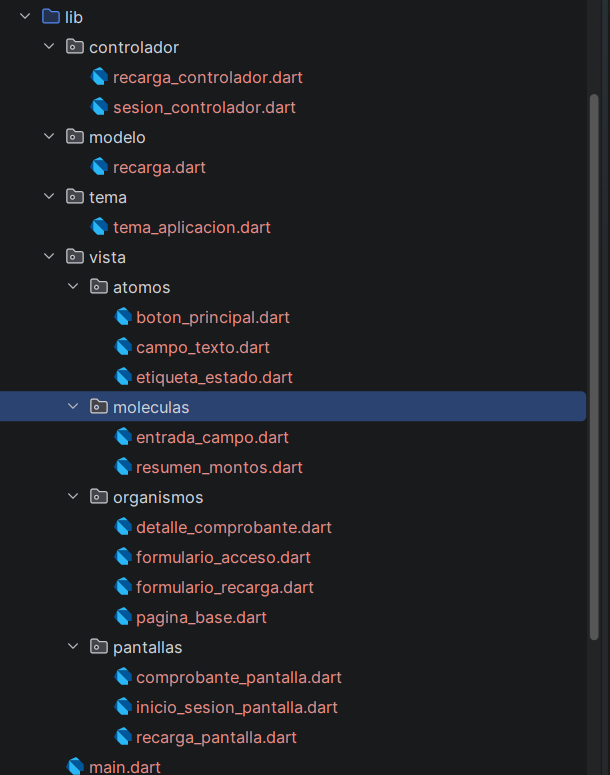
\includegraphics[width=\linewidth,height=11.7cm,keepaspectratio]{images/estructura_proyecto.png}\par}
\vspace{6pt}
\noindent\textit{Nota.} La captura muestra la organización del modelo, los controladores, el tema y los componentes de la vista.
\end{figure}


\texttt{SesionControlador} valida las credenciales y mantiene el usuario de la sesión. \texttt{RecargaControlador} valida los datos de recarga, produce una cotización y genera el comprobante. En el modelo, \texttt{Operadora} define las tasas simuladas, \texttt{FormaPago} limita las alternativas y \texttt{Comprobante} conserva una instantánea inmutable de la operación.

\begin{figure}[H]\caption{Relación entre las responsabilidades MVC}\label{fig:mvc}
\centering
\begin{tikzpicture}[every node/.style={draw,rounded corners,align=center,text width=3.5cm,minimum height=1.5cm,font=\small},>=Stealth]
\node (vista) {Vista\\Formularios y pantallas};
\node[right=0.8cm of vista] (control) {Controlador\\Validación y coordinación};
\node[right=0.8cm of control] (modelo) {Modelo\\Cotización y comprobante};
\draw[->] (vista) -- (control);\draw[->] (control) -- (modelo);
\end{tikzpicture}
\par\raggedright\noindent\textit{Nota.} Diagrama elaborado a partir de la organización del código. Las vistas reciben los resultados del controlador y los presentan; el modelo no importa widgets.
\end{figure}

\begin{table}[H]\centering
\caption{Aplicación de Atomic Design en los componentes}\label{tab:atomic}
\begin{tabular}{@{}p{2.5cm}p{5.5cm}p{5.2cm}@{}}\toprule
Nivel & Componentes & Responsabilidad \\\midrule
Átomos & CampoTexto, BotonPrincipal, EtiquetaEstado & Entrada, acción y distintivo básicos \\
Moléculas & EntradaCampo, ResumenMontos & Entrada con contexto y resumen monetario \\
Organismos & FormularioAcceso, FormularioRecarga, DetalleComprobante, PaginaBase & Bloques completos de interfaz \\
Pantallas & InicioSesionPantalla, RecargaPantalla, ComprobantePantalla & Composición y acciones de cada destino \\\bottomrule
\end{tabular}
\notatabla{\texttt{EntradaCampo} utiliza el átomo \texttt{CampoTexto}; los formularios reutilizan las moléculas y los botones.}
\end{table}

\subsubsection{Paso 2 Creación del proyecto y del tema}
Se creó el proyecto con soporte Android y web y se mantuvieron únicamente las dependencias de ejecución del SDK. La plataforma Android se utilizó para la ejecución documentada; la carpeta web queda disponible como destino del proyecto, sin atribuirle una prueba Android.
\begin{lstlisting}
flutter create --platforms=android,web --org ec.edu.espe --project-name recargas_espe --empty recargas_espe
\end{lstlisting}
El archivo \texttt{tema/tema\_aplicacion.dart} concentra el tema claro. Se utilizaron verde \texttt{\#135E4B}, fondo \texttt{\#F4F6F2} y texto \texttt{\#182D26}. Los botones principales mantienen un tamaño mínimo de 52 unidades lógicas y los campos comparten bordes, relleno y espacio interno. \texttt{PaginaBase} aporta desplazamiento vertical y limita el ancho del contenido en superficies grandes.

\subsubsection{Paso 3 Implementación del inicio de sesión}
La primera pantalla incluye usuario, contraseña, control para mostrar u ocultar su contenido, botón Iniciar sesión y botón Limpiar. La validación distingue dos casos: campos vacíos, que muestran un mensaje asociado al campo, y credenciales incorrectas, que generan un mensaje general sin navegar. Al ingresar las credenciales válidas se abre la pantalla de recarga.

El botón Limpiar elimina los textos, los errores y la visibilidad temporal de la contraseña. Las credenciales se muestran como acceso de práctica para facilitar la evaluación. Al estar definidas dentro del código, este mecanismo sirve al ejercicio y no constituye autenticación apta para un servicio real.
\pantalla{01_acceso.png}{Pantalla de inicio de sesión}{fig:acceso}{Se observan los dos campos, el control de visibilidad y las acciones de acceso y limpieza.}
\pantalla{02_validacion_acceso.png}{Validación de campos vacíos en el acceso}{fig:accesovacio}{La solicitud de acceso sin datos mantuvo la pantalla y mostró los mensajes correspondientes.}
\pantalla{03_credenciales_incorrectas.png}{Respuesta ante credenciales incorrectas}{fig:accesoincorrecto}{El mensaje informa el rechazo del acceso; no se abrió la pantalla principal.}

\subsubsection{Paso 4 Implementación de la nueva recarga}
La segunda pantalla solicita número telefónico, operadora, valor en dólares y forma de pago. El teléfono se captura con teclado telefónico y el monto con teclado numérico decimal; ambos se validan nuevamente mediante las reglas del controlador. Los selectores limitan la operadora y el pago a las opciones definidas.

Al modificar el monto o la operadora se actualiza la cotización visible, sin crear todavía un comprobante. La confirmación solo continúa cuando todo el formulario es válido. Limpiar recarga restablece texto, selecciones y resultado. El resumen presenta valor, comisión y total, para que la persona pueda revisar el cálculo antes de continuar.
\pantalla{04_nueva_recarga.png}{Formulario principal de nueva recarga}{fig:recargavacia}{Las selecciones comienzan vacías y el resumen inicial muestra valores de cero.}

\subsubsection{Paso 5 Cálculo de la comisión y redondeo}
Para una recarga de valor $V$ y una tasa de comisión $p$, la lógica corresponde a:
\[
C=V\times p,\qquad T=V+C.
\]
En la implementación, $v$ representa el valor en centavos y $b$ la tasa en puntos base. La comisión entera se calcula con:
\[
c=\left\lfloor\frac{v\times b+5000}{10000}\right\rfloor,
\qquad t=v+c.
\]
La adición de 5000 aplica el redondeo de mitad hacia arriba para importes positivos. Por ejemplo, USD 1,00 con Movistar produce USD 0,025 de comisión antes de redondear; el comprobante registra USD 0,03 y un total de USD 1,03. No se redondea el monto de entrada: si contiene más de dos decimales, se rechaza.

\begin{table}[H]\centering
\caption{Resultados esperados para una recarga de diez dólares}\label{tab:comisiones}
\begin{tabular}{@{}p{3.4cm}p{2.4cm}p{3.4cm}p{3.4cm}@{}}\toprule
Operadora & Comisión & Valor de comisión & Total a pagar \\\midrule
Claro & 3\% & USD 0,30 & USD 10,30 \\
Movistar & 2,5\% & USD 0,25 & USD 10,25 \\
CNT & 2\% & USD 0,20 & USD 10,20 \\\bottomrule
\end{tabular}
\notatabla{Los tres casos se verificaron con pruebas unitarias. La Figura~\ref{fig:recargalista} documenta el caso Claro en la interfaz Android.}
\end{table}
\pantalla{05_recarga_claro.png}{Cotización de una recarga de diez dólares con Claro}{fig:recargalista}{La interfaz presenta USD 0,30 de comisión y USD 10,30 de total antes de confirmar.}

\subsubsection{Paso 6 Comprobante y navegación por rutas}
La tercera pantalla presenta teléfono, operadora, pago, usuario, fecha local, identificador, valor, comisión y total. El código se forma con una marca temporal y una secuencia en memoria; distingue operaciones durante la sesión del proceso, sin afirmar unicidad entre instalaciones. El texto indica que la operación es una simulación.

En \texttt{main.dart} se definieron las rutas \texttt{/}, \texttt{/recarga} y \texttt{/comprobante}. El generador de rutas comprueba la sesión antes de presentar pantallas internas. El destino del comprobante requiere un resultado disponible; si no existe, se presenta el formulario. La acción Nueva recarga elimina el comprobante anterior y abre un formulario nuevo. Cerrar sesión elimina usuario y resultado, y reemplaza la pila de navegación con el acceso.
\pantalla{06_comprobante.png}{Comprobante de la operación simulada}{fig:comprobante}{El resultado conserva los datos confirmados y permite comenzar una nueva recarga. El teléfono se utilizó únicamente como dato de prueba y no fue contactado.}

\subsection{Pruebas}
\subsubsection{Estrategia y ejecución}
Se ejecutaron pruebas unitarias de controladores y modelos, y pruebas de widgets que interactúan con la aplicación. La primera prueba de acceso falló sobre el proyecto vacío, porque todavía no existían sus controles. Después de implementarlos se verificó el comportamiento funcional, sin sustituirlo por capturas de una maqueta.

La suite final comprende 30 pruebas unitarias y siete pruebas de widgets, para un total de 37. Las primeras comprueban credenciales, formatos, límites, tasas, redondeo, creación y limpieza del comprobante. Las segundas verifican controles obligatorios, mensajes, visibilidad de contraseña, limpieza, protección de ruta, flujo completo y adaptación a pantalla estrecha.
\begin{lstlisting}
flutter analyze
flutter test --reporter expanded
flutter build apk --debug
\end{lstlisting}

\subsubsection{Casos y criterios de aceptación}
\begin{table}[H]\centering
\caption{Resumen de las comprobaciones funcionales}\label{tab:pruebas}
\small
\begin{tabular}{@{}p{1cm}p{6.7cm}p{7.7cm}@{}}\toprule
Caso & Entrada o acción & Criterio comprobado \\\midrule
P01 & Acceso vacío & Mensajes en usuario y contraseña; sin navegación \\
P02 & Contraseña incorrecta & Rechazo del acceso \\
P03 & Credenciales de práctica & Apertura del formulario principal \\
P04 & Mostrar y limpiar contraseña & Cambio de visibilidad y reinicio de campos \\
P05 & Teléfono incompleto o inválido & Rechazo por formato \\
P06 & Monto negativo, texto o más de dos decimales & Rechazo de la entrada \\
P07 & Montos 1,00 y 100,00 & Aceptación de ambos límites \\
P08 & Montos 0,99 y 100,01 & Rechazo fuera del rango \\
P09 & Diez dólares por operadora & Totales 10,30; 10,25 y 10,20 \\
P10 & Un dólar con Movistar & Comisión 0,03 tras redondear \\
P11 & Confirmar sin selecciones & Permanencia en el formulario y errores \\
P12 & Recarga completa y Nueva recarga & Comprobante correcto y formulario limpio \\
P13 & Ruta interna sin sesión & Presentación del acceso \\
P14 & Pantalla de 320 por 640 y texto al 150\% & Desplazamiento sin desbordamientos detectados \\\bottomrule
\end{tabular}
\notatabla{La tabla agrupa comportamientos; no equivale al número de funciones de prueba. Los resultados se verificaron mediante la suite automatizada.}
\end{table}

\subsubsection{Recorrido en Android}
Se compiló el APK de depuración y se ejecutó en el emulador indicado en la Tabla~\ref{tab:entorno}. Una prueba de integración Android adicional recorrió acceso vacío, credenciales incorrectas, acceso válido, formulario de recarga, comprobante, nueva operación y cierre de sesión. Las Figuras~\ref{fig:acceso} a~\ref{fig:comprobante} se capturaron directamente desde la interfaz ejecutada mediante \texttt{integration\_test} y se conservaron como archivos PNG. Esta prueba de integración es adicional a las 37 pruebas unitarias y de widgets.
\begin{lstlisting}
flutter drive --driver=test_driver/integration_test.dart --target=integration_test/recorrido_test.dart -d emulator-5554
\end{lstlisting}

La captura de la interfaz acredita el estado visible en ese momento. Las comprobaciones del cálculo para otras operadoras y de entradas límite se respaldan con las pruebas automatizadas, sin presentar una captura de Claro como evidencia visual de las otras tasas.

\subsubsection{Resultados y análisis}
El análisis estático finalizó sin incidencias y la suite automatizada registró 37 pruebas aprobadas. La compilación Android produjo un APK de depuración. El recorrido en el emulador mostró las tres pantallas y un comprobante de USD 10,30 para una recarga de USD 10,00 con comisión del 3\%.

La estructura de carpetas permite identificar dónde modificar cada comportamiento. Cambiar una tasa afecta al modelo; modificar la validación afecta al controlador; ajustar un campo compartido afecta a sus componentes visuales. La composición evita repetir el formulario de acceso en otra pantalla y reutiliza el resumen monetario en la cotización y el comprobante.

\begin{table}[H]\centering
\caption{Correspondencia entre requisitos y evidencias}\label{tab:cumplimiento}
\begin{tabular}{@{}p{4.1cm}p{5.3cm}p{3.8cm}@{}}\toprule
Requisito & Implementación & Evidencia \\\midrule
Tres pantallas funcionales & Acceso, recarga y comprobante & Figuras~\ref{fig:acceso} a~\ref{fig:comprobante} \\
MVC & modelo, controlador y vista & Figura~\ref{fig:mvc} y código \\
Atomic Design & Cuatro niveles dentro de vista & Tabla 3 y código \\
Tema propio & tema\_aplicacion.dart & Capturas Android \\
Rutas & main.dart y RutasApp & Prueba del flujo y de acceso \\
Validación de entradas & Controladores y Form & Tabla 5 y suite de pruebas \\
Comisiones diferentes & Tasas por Operadora & Tabla 4 y pruebas unitarias \\
Acceso con controles requeridos & FormularioAcceso & Figuras~\ref{fig:acceso} a~\ref{fig:accesoincorrecto} y widgets \\\bottomrule
\end{tabular}
\notatabla{La evidencia combina inspección del código, pruebas y ejecución. Cada método acredita una parte del requisito.}
\end{table}

\subsubsection{Registro de incidencias}
Durante la verificación se detectó que el título del encabezado y el selector de pago desbordaban su espacio en una pantalla de 320 unidades de ancho con texto ampliado al 150\%. El título se hizo flexible y se habilitó la expansión del selector dentro del ancho disponible. La prueba se repitió y finalizó sin excepciones de diseño. También se corrigió la consulta de visibilidad de contraseña en la prueba: esa propiedad se comprueba en el \texttt{TextField} interno, no en \texttt{TextFormField}.

\subsubsection{Alcance de la verificación}
Los resultados acreditan las reglas e interacciones cubiertas por la suite y el funcionamiento observado en un emulador Android. No constituyen pruebas de carga, una auditoría completa de accesibilidad, mediciones de rendimiento ni validación en todos los tamaños y dispositivos. La autenticación es local y el comprobante no tiene validez comercial. No se implementaron servidor, base de datos, historial persistente, pagos ni servicios de recarga reales.

\section{Conclusiones}
\begin{enumerate}[leftmargin=*]
\item Se desarrolló una aplicación de recargas con las tres pantallas requeridas y un flujo completo desde el acceso hasta el comprobante. Los datos ingresados se validan antes de confirmar y los mensajes permiten identificar errores sin avanzar a una operación incompleta.
\item La aplicación combinó MVC con Atomic Design. Las carpetas en español conservan el enfoque trabajado en clase y separan las reglas de negocio de los componentes de presentación. El tema compartido mantuvo colores, tipografía y controles consistentes.
\item Las tasas diferenciadas y el cálculo en centavos produjeron resultados reproducibles, incluido el redondeo de medio centavo. Las 37 pruebas aprobadas, el análisis estático sin incidencias y el recorrido Android respaldan el alcance funcional descrito, sujeto a los límites de la simulación.
\end{enumerate}

\section{Recomendaciones}
\begin{enumerate}[leftmargin=*]
\item Mantener las tasas de práctica identificadas como valores simulados. Si la aplicación se conecta posteriormente con una operadora o un sistema de pagos, reemplazar la validación local por autenticación de servidor y verificar las reglas del servicio antes de procesar operaciones.
\item Conservar la separación de responsabilidades al agregar funciones y ejecutar las pruebas cuando cambien límites, tasas o navegación. Ampliar la verificación a dispositivos físicos, más escalas de texto y otras versiones de Android antes de plantear una distribución.
\item Conservar las capturas de las comprobaciones y repetir las pruebas antes de modificar las reglas de negocio. Una distribución futura requeriría configurar y firmar una versión de publicación.
\end{enumerate}

\begin{thebibliography}{15}
\bibitem[Bia{\l}kowski y Smo{\l}ka(2022)]{bialkowski2022}
Bia{\l}kowski, D., \& Smo{\l}ka, J. (2022). Evaluation of Flutter framework time efficiency in context of user interface tasks. \textit{Journal of Computer Sciences Institute, 25}, 309--314. \url{https://doi.org/10.35784/jcsi.3007}

\bibitem[Bi{\o}rn-Hansen et~al.(2020)]{biornhansen2020}
Bi{\o}rn-Hansen, A., Rieger, C., Gr{\o}nli, T.-M., Majchrzak, T. A., \& Ghinea, G. (2020). An empirical investigation of performance overhead in cross-platform mobile development frameworks. \textit{Empirical Software Engineering, 25}(4), 2997--3040. \url{https://doi.org/10.1007/s10664-020-09827-6}

\bibitem[Dart(s. f.)]{darttipos}
Dart. (s. f.). \textit{Built-in types}. Recuperado el 2 de noviembre de 2026, de \url{https://dart.dev/language/built-in-types}

\bibitem[Flutter(s. f.-a)]{flutteride}
Flutter. (s. f.-a). \textit{Android Studio and IntelliJ}. Recuperado el 2 de noviembre de 2026, de \url{https://docs.flutter.dev/tools/android-studio}

\bibitem[Flutter(s. f.-b)]{flutterformularios}
Flutter. (s. f.-b). \textit{Build a form with validation}. Recuperado el 2 de noviembre de 2026, de \url{https://docs.flutter.dev/cookbook/forms/validation}

\bibitem[Flutter(s. f.-c)]{flutterselector}
Flutter. (s. f.-c). \textit{DropdownButtonFormField class}. Recuperado el 2 de noviembre de 2026, de \url{https://api.flutter.dev/flutter/material/DropdownButtonFormField-class.html}

\bibitem[Flutter(s. f.-d)]{flutterarquitectura}
Flutter. (s. f.-d). \textit{Flutter architectural overview}. Recuperado el 2 de noviembre de 2026, de \url{https://docs.flutter.dev/resources/architectural-overview}

\bibitem[Flutter(s. f.-e)]{flutterrutas}
Flutter. (s. f.-e). \textit{Navigate with named routes}. Recuperado el 2 de noviembre de 2026, de \url{https://docs.flutter.dev/cookbook/navigation/named-routes}

\bibitem[Flutter(s. f.-f)]{flutterpruebas}
Flutter. (s. f.-f). \textit{Testing Flutter apps}. Recuperado el 2 de noviembre de 2026, de \url{https://docs.flutter.dev/testing/overview}

\bibitem[Flutter(s. f.-g)]{fluttertema}
Flutter. (s. f.-g). \textit{Use themes to share colors and font styles}. Recuperado el 2 de noviembre de 2026, de \url{https://docs.flutter.dev/cookbook/design/themes}

\bibitem[Frost(s. f.)]{frost}
Frost, B. (s. f.). Atomic design methodology. En \textit{Atomic design}. \url{https://atomicdesign.bradfrost.com/chapter-2/}

\bibitem[Jo\v{s}t y Taneski(2025)]{jost2025}
Jo\v{s}t, G., \& Taneski, V. (2025). State-of-the-art cross-platform mobile application development frameworks: A comparative study of market and developer trends. \textit{Informatics, 12}(2), Artículo 45. \url{https://doi.org/10.3390/informatics12020045}

\bibitem[MDN Web Docs(s. f.)]{mdnmvc}
MDN Web Docs. (s. f.). \textit{MVC}. Recuperado el 2 de noviembre de 2026, de \url{https://developer.mozilla.org/en-US/docs/Glossary/MVC}

\bibitem[Rieger y Majchrzak(2019)]{rieger2019}
Rieger, C., \& Majchrzak, T. A. (2019). Towards the definitive evaluation framework for cross-platform app development approaches. \textit{Journal of Systems and Software, 153}, 175--199. \url{https://doi.org/10.1016/j.jss.2019.04.001}

\bibitem[Uci\'{n}ski y Dzie\'{n}kowski(2022)]{ucinski2022}
Uci\'{n}ski, M., \& Dzie\'{n}kowski, M. (2022). A comparative analysis of performance of Flutter and Xamarin development frameworks. \textit{Journal of Computer Sciences Institute, 25}, 366--370. \url{https://doi.org/10.35784/jcsi.3025}

\end{thebibliography}

\end{document}
